%%%%%%%%%%%%%%%%%%%%%%%%%%%%%%%%%%%%%%%%%%%%%%
%                insertmeeting
% 1) Title (something creative & funny?)
% 2) Date (MM/DD/YYYY)
% 3) Location (ex. Hagerty High School)
% 4) People/Committees Present 
% 5) Picture 
% 6) Start Time & Stop Time (ex. 12:30AM to 4:30PM)
%%%%%%%%%%%%%%%%%%%%%%%%%%%%%%%%%%%%%%%%%%%%%%
\insertmeeting 
	{Tricky Tricycles and Smooth Scriptwriting} 
	{01/06/22} 
	{Hagerty High School}
	{Annika, Anouska, Clayton, Falon, James, Jensen, Nathan, Ritam, Rose, Samantha}
	{Images/RobotPics/robot.jpg}
	{2:30 - 4:30}
	
\hhscommittee{Software}
\noindent\hfil\rule{\textwidth}{.4pt}\hfil
\subsubsection*{Goals}
\begin{itemize}
    \item Explore Localization Methods for Tricycle Drivebases

\end{itemize} 

\noindent\hfil\rule{\textwidth}{.4pt}\hfil

\subsubsection*{Accomplishments}
We started today with quick Google searches for general localization. We found a lot of resources for localization on robots with four wheels. These systems worked for both holonomic and differential drive bases. However, our three wheeled robot didn't exactly fit into either category. However, we did learn a lot about the fundamental principles used in localization. Essentially, we should be trying to find the distance the center of the robot traveled by taking the average of the change in left and right encoders. After taking these measurements, we should be able to use them in kinematic equations to figure out how the robot is traveling relative to the field. Our focus should be taking our encoder readings, which are in one dimension, and use trig functions and kinematic equations to convert them into field coordinates that can be used with Road Runner and other autonomous applications. 

\begin{figure}[htp]
\centering
  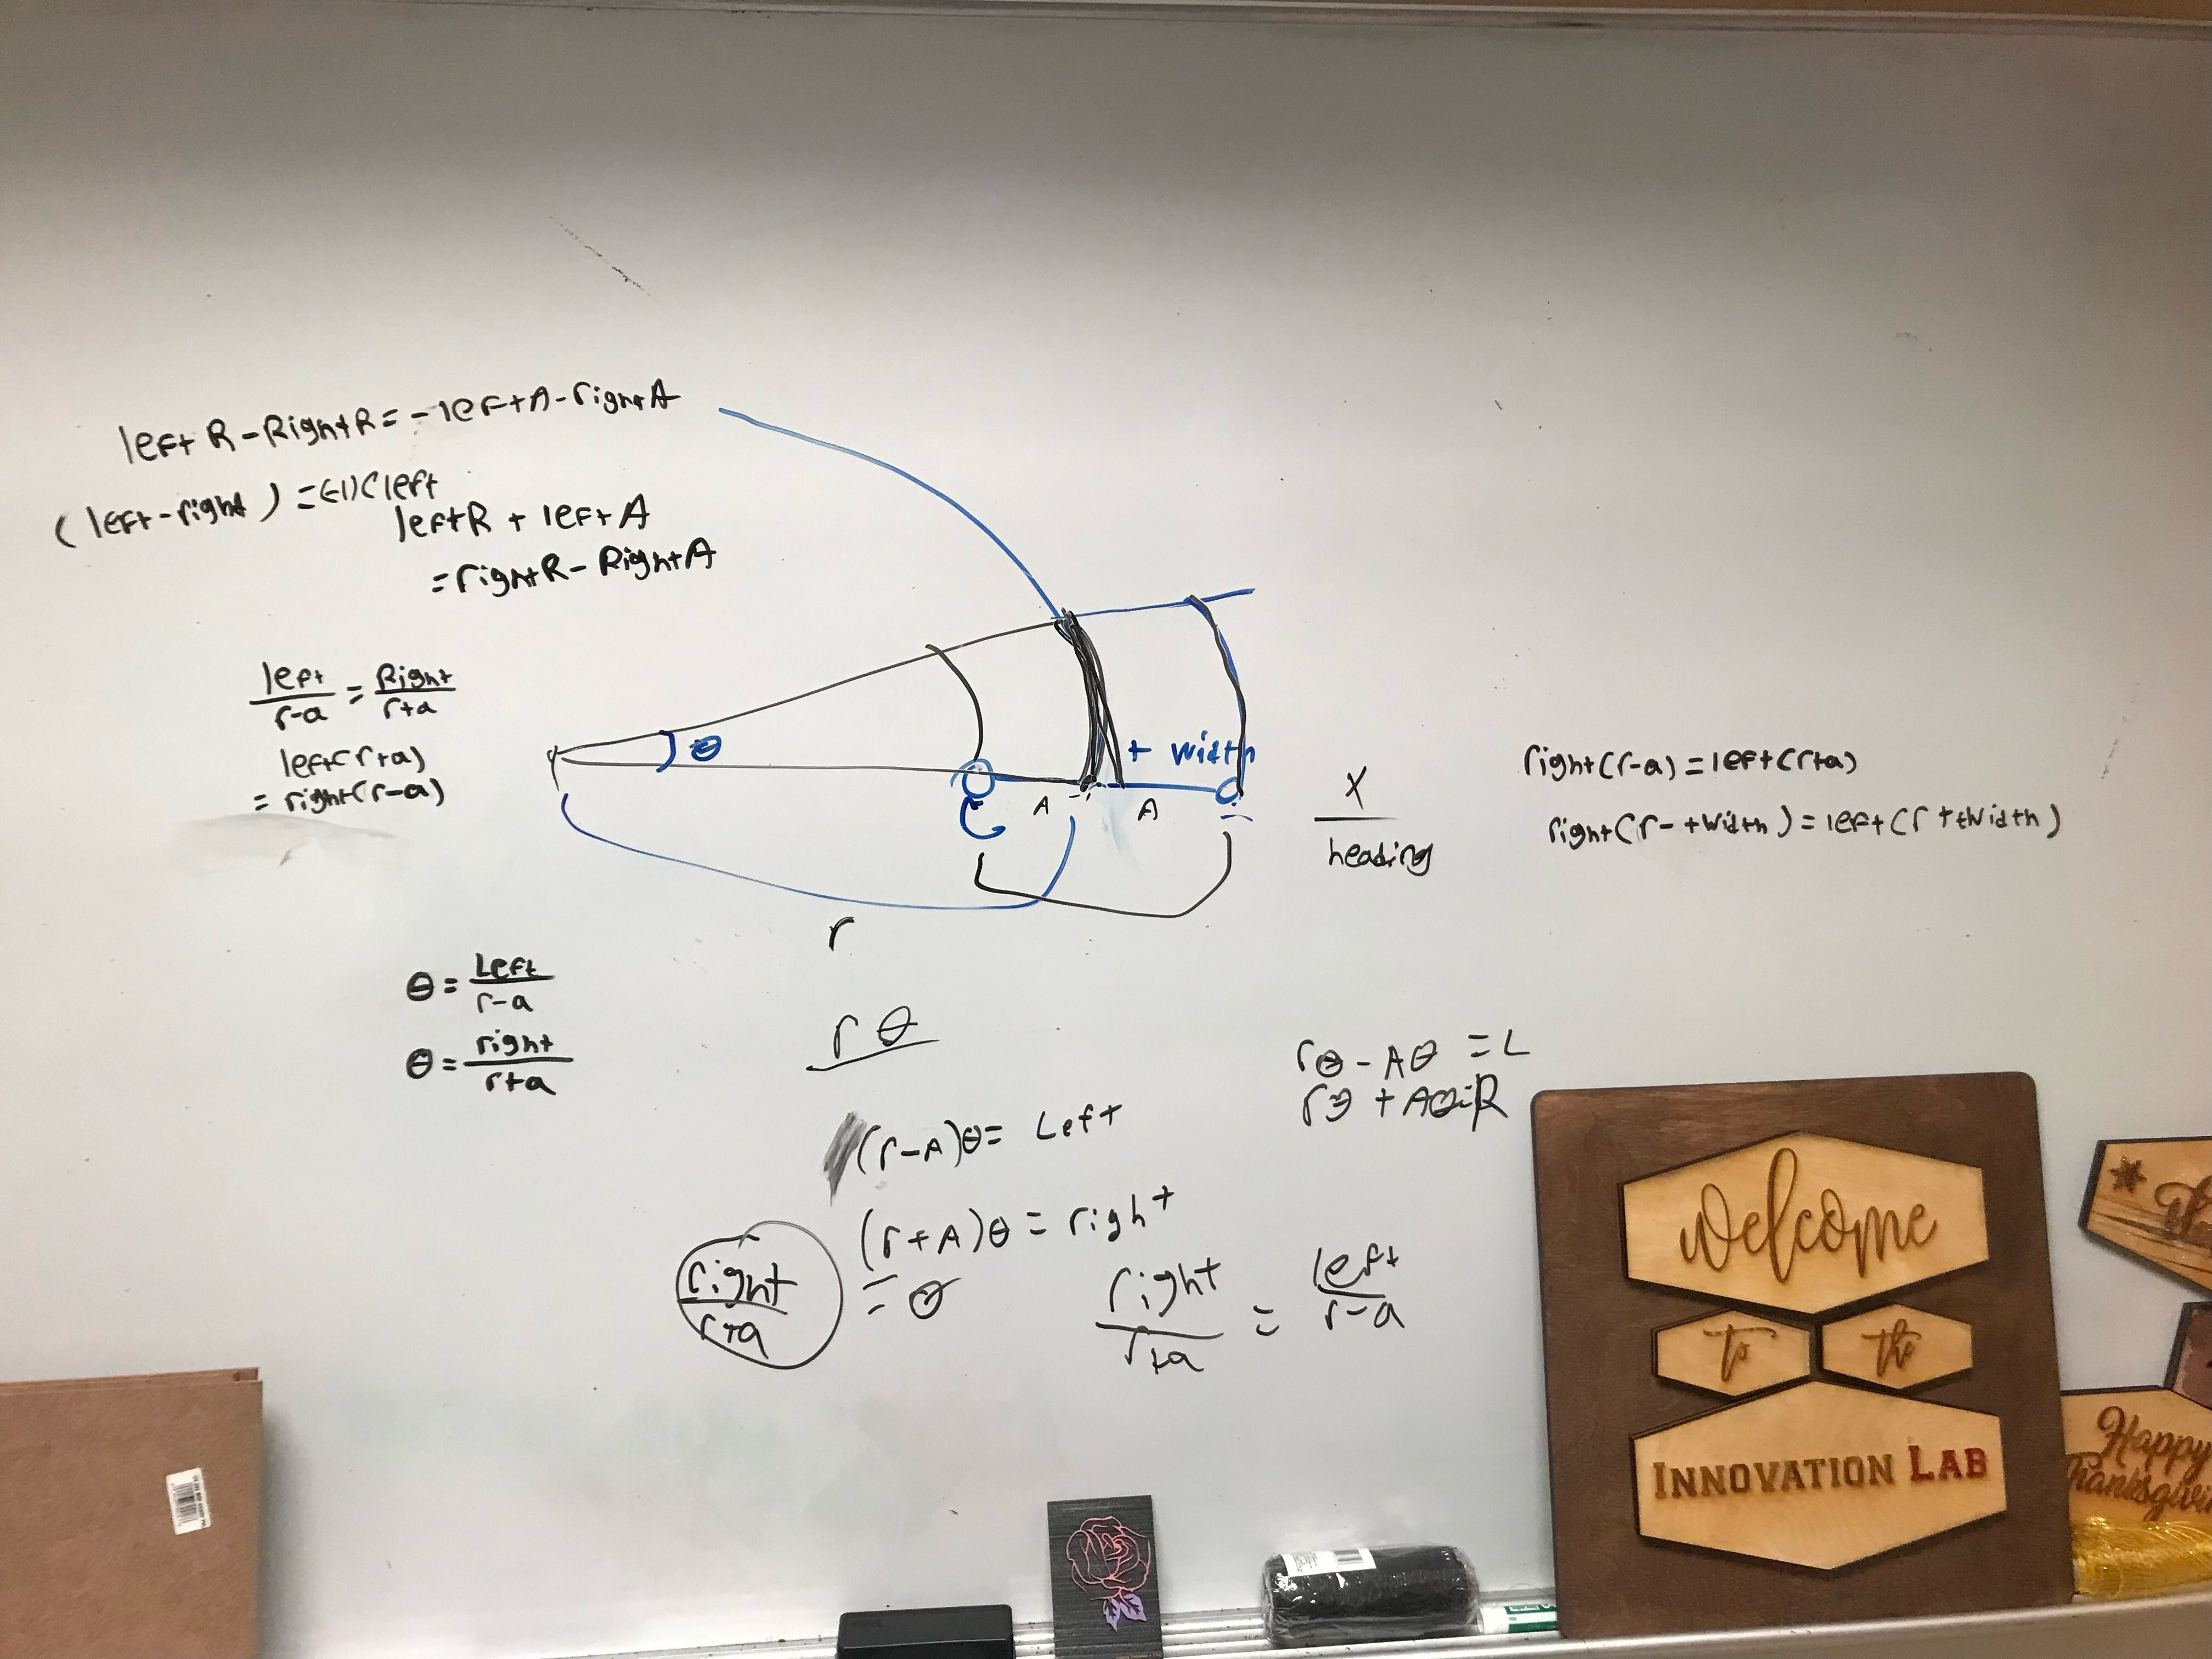
\includegraphics[width=0.95\textwidth]{Meetings/January/01-06-22/1.6.22 Board with Odometry - James Hu.jpg}
  \caption{Whiteboard showing our ideas on approaching tricycle odometry}
  \label{fig:010622_1}
\end{figure}

\begin{figure}[htp]
\centering
  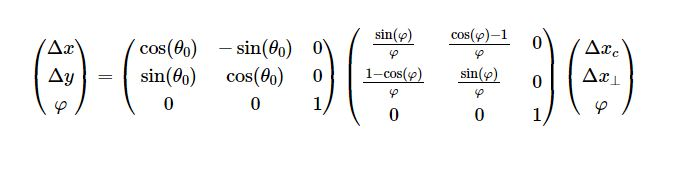
\includegraphics[width=0.95\textwidth]{Meetings/January/01-06-22/1.6.22 Corrected Pose Equation - James Hu.JPG}
  \caption{A screenshot from GM0 on transforming robot-centric coordinates into field-centric coordinates}
  \label{fig:010622_2}
\end{figure}

\hhscommittee{Multimedia}
\noindent\hfil\rule{\textwidth}{.4pt}\hfil
\subsubsection*{Goals}
\begin{itemize}
    \item We will finish the video script today for the Promote video. We will also try to start drawing out visual storyboards for the video.

\end{itemize} 

\noindent\hfil\rule{\textwidth}{.4pt}\hfil

\subsubsection*{Accomplishments}
During today's meeting, the multimedia committee was focused primarily on script-writing. Following today's meeting, we will have under a month to complete the video, so we need to start picking up the pace. We decided to structure the script in the form of a letter, beginning with "Dear Little Me," to stay address the prompt of what we would tell our younger selves about FIRST. The script is divided according to each main scene of the video, which follows the life of the Little Fire Guy character as it progresses through each stage of its life while involved in FIRST. We decided to conclude the script by directly addressing the prompt, and responding to it. By doing this, we believe that the viewer will remember this line best and heed our advice to "take the wheel". In the context of our Promote video, this basically means 'take initiative'. We were inspired by this year's transportation theme, hence the reference to a steering wheel. We made good progress today and have written out the entire script.

\whatsnext{
\begin{itemize}
    \item During tomorrow's meeting, we will revise the script and make changes. We will get some peer review on it and edit it accordingly.
    \item Focus on deriving formulas for tricycle drives. 
\end{itemize} 
}

